\section{费马小定理的组合证明}
\phantomsection
\label[appendix]{app:fermat-little-theorem}

我们再介绍费马小定理的一种组合证明方法。%% \cite{Wiki-FLT-proof}

\begin{proof}
考虑有$a$种不同颜色的珍珠,我们要串一条长为$p$的珍珠串。其中$p$为素数。显然一共有$a^p$种不同的串,这是因为串中每个位置都可以在$a$种颜色的珍珠中选择,共选$p$次。

例如有两种颜色$A$红、$B$绿的珍珠,要串长度为5的串。即$a = 2, p = 5$,一共有$2^5 = 32$种不同的串:

\begin{verbatim}
  AAAAA, AAAAB, AAABA, ..., BBBBA, BBBBB.
\end{verbatim}

对应:红红红红红, 红红红红绿, 红红红绿红, ..., 绿绿绿绿红, 绿绿绿绿绿.

我们要证明,在这$a^p$串珍珠中,如果去掉$a$个颜色完全相同的串(在上述例子中是串\texttt{AAAAA}和\texttt{BBBBB}),剩下的$a^p - a$串珍珠可以分成若干组,每个组恰好有$p$串珍珠。也就是说$p$整除$a^p - a$。

如果把每串珍珠首尾连接起来做成项链。原来有些不同的串会变成相同的项链。如果一个串可以通过旋转变换成另一个,这两个串必然做成相同的项链。例如下面的5串珍珠可以做成相同的项链:

\begin{verbatim}
  AAAAB, AAABA, AABAA, ABAAA, BAAAA.
\end{verbatim}

\begin{figure}[htbp]
  \centering
  \subcaptionbox{一串含3种颜色的项链代表7种不同的串:\texttt{ABCBAAC}, \texttt{BCBAACA}, \texttt{CBAACAB}, \texttt{BAACABC}, \texttt{AACABCB}, \texttt{ACABCBA}, \texttt{CABCBAA}}[0.45\linewidth]{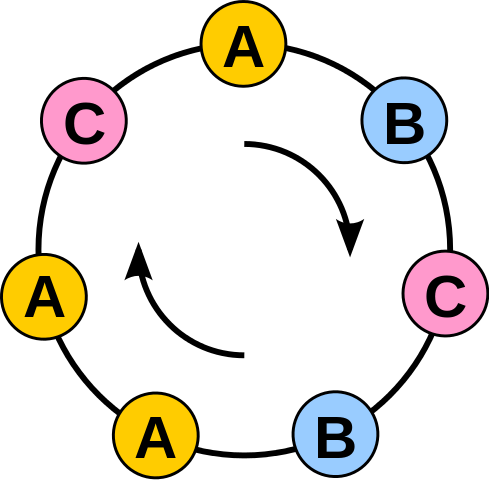
\includegraphics[scale=0.2]{../img/bracelet-rotate}} \quad
  \subcaptionbox{相同颜色珍珠串成的项链只代表一种串:\texttt{AAAAAAA}}[0.45\linewidth]{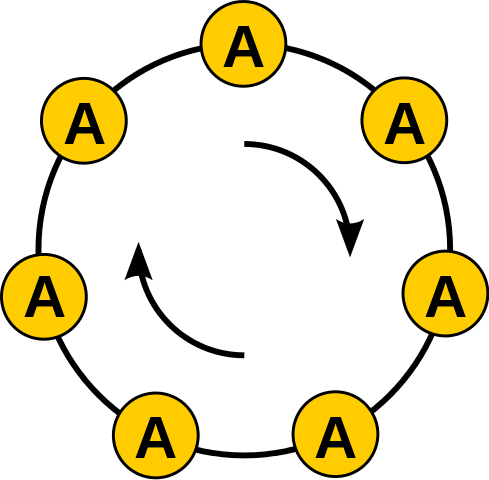
\includegraphics[scale=0.2]{../img/bracelet-identical}}
  \caption{通过项链对珍珠串进行分类}
  \label{fig:bracelet}
\end{figure}

用这种方法,上面例子中的32串珍珠可以分成5种不同颜色的项链和2种同色的项链:

\begin{verbatim}
  [AAABB, AABBA, ABBAA, BBAAA, BAAAB];
  [AABAB, ABABA, BABAA, ABAAB, BAABA];
  [AABBB, ABBBA, BBBAA, BBAAB, BAABB];
  [ABABB, BABBA, ABBAB, BBABA, BABAB];
  [ABBBB, BBBBA, BBBAB, BBABB, BABBB];
  [AAAAA];
  [BBBBB].
\end{verbatim}

一串项链可以代表多少种不同的串呢?如果一个串$S$由若干相同的子串$T$复制连接而成,而$T$无法再继续分拆成相同的子串,则由$S$构成的项链可代表$|T|$种不同的串,其中$|T|$表示串$T$的长度。例如串$S=$\texttt{ABBABBABBABB},由相同的子串$T=$\texttt{ABB}复制多次而成,如果我们一次旋转一颗珍珠,一共可以得到3串不同的结果:

\begin{verbatim}
  ABBABBABBABB,
  BBABBABBABBA,
  BABBABBABBAB.
\end{verbatim}

除去这3种之外,不可能再有其它不同种类的串了。\texttt{ABB}的长度为3,再次旋转必然会循环得到相同的结果。这样,所有的$a^p$串珍珠可分成两类。一类是$a$串颜色相同的串;另一类颜色不同,但是由于这些串的长度$p$是素数,它绝不可能由若干子串复制连接出来。所以任何一个这样的串连成的项链,总共代表$p$种不同的串。而这样的串总共有$a^p - a$种,它们可以通过连成项链后分组,每组恰好$p$个串,代表一种不同的项链。因此$a^p-a = a(a^{p-1}-1)$一定可以被$p$整除。由于$a$和$p$互素,所以$p$一定整除$a^{p-1}-1$。
\end{proof}

组合证明法不需要太多的数学知识。核心思想是利用两种不同的方式数数的结果必然是一样的。
